\section{The Large Hadron Collider}

Located in the Lemanic basin, straddling the border between Switzerland and France, the Large Hadron Collider is the largest machine built by humans.
The LHC provides the unique laboratory conditions in which detectors like ATLAS investigate the fundamental nature of our Universe.
The construction, maintenance, and operation of the LHC are part of an enormous effort carried out by thousands of dedicated scientists and engineers. Without their ongoing endeavors, the achievements of ATLAS and the other LHC experiments would be impossible.

The LHC is impressive not just in absolute terms, but also in comparison to previous accelerators.
The three other large superconducting accelerators, the Tevatron\footnote{Decommissioned in 2011.}, HERA\footnote{Decommissioned in 2007}, and RHIC, all operate with fields of approximately 5~T. The LHC exceeds this with fields of 8~T.
The machine is also enormous; it has a circumference of 26.7~km. It takes 15 days to cool down a sector.
The LHC, designed to reach collision energies of 14 TeV, is also the first hadron accelerator with enough synchrotron radiation to affect the design of the cooling and vacuum systems \cite{lyndon}.

The LHC is composed of several subsystems, each of which is complex and essential in its own right.
In particular, the following systems will be described here:
\begin{itemize}
    \item The magnet system, which is responsible for bending the beam around the path of the machine.
    \item The vacuum system, which evacuates the beampipe.
    \item The radio-frequency system, which accelerates the beams. 
    \item The power system that powers the machine.
    \item The beam instrumentation, collimation, and control systems that monitor and adjust the beam.
    \item The beam injection and extraction systems.
\end{itemize}
The LHC is a machine under continuous development. The only place to study improvements for the LHC is at the LHC.
As a result, the history of the LHC development is also the history of the experimental environment of the ATLAS detector.
This story begins with the tunnel and infrastructure that houses the LHC.

\subsection{Civil Engineering}

\begin{figure}[h!]
\captionsetup[subfigure]{position=b}
\centering
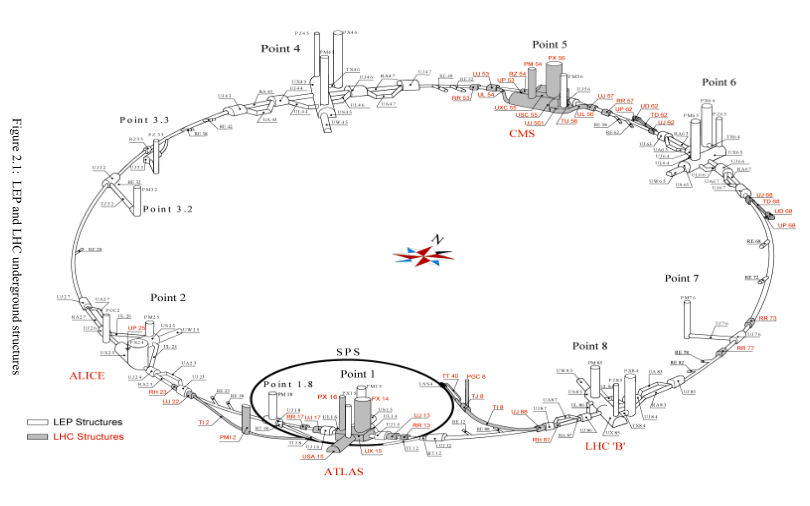
\includegraphics[width=0.9\textwidth]{figures/experiment/lhcLepLayout.png}
\caption{The LHC infrastructure layout. Figure from the LHC Design Report \cite{lhcDesignV2}.}
\label{figure:lhcLayout}
\end{figure}


The first step in building a collider is civil infrastructure.
This takes the form of a building that houses services for the accelerator and a space for the machine itself.
For economic reasons, much of the infrastructure for the LHC is reused from the earlier LEP project.

The largest piece of infrastructure is the tunnel built to house LEP.
The Tevatron is buried less than 10~m deep in the flat expanse of the Illinois prairie. This shallow tunnel could be constructed with a cut-and-fill approach.
RHIC is primarily built at surface level in a tunnel that was later covered with dirt.
Neither of these approaches was suitable in the context of the geology of the region.
The land near CERN consists of a layer of moraine (loose unconsolidated rock) resting atop a layer of molasse (soft sedimentary rock).
LEP was buried in the sedimentary layer for stability, but this is too deep for excavation.
Instead, beginning in 1985, the tunnel was dug using tunnel bores and explosives.
In the Cenozoic molasse of the Lemanic basin, tunnel bores were the fastest option.
The tunnel bores were unsuitable for the fractured Mesozoic limestone beneath the Jura mountain, and explosives were used instead.
The resulting tunnel's internal diameter is 3.8~m, and it is buried at a depth of 45-170~m.
The tunnel slopes downward at 1.42 degrees in the direction of Lake Leman, in order to remain within the molasse layer.

The tunnel has eight curved arcs, separated by eight straight sections with length 528~m. \cite{lyndon}
Four straight sections house the ATLAS, CMS, ALICE, and LHCb experiments. These are 
The other four straight sections house the RF system, collimation controls, beam abort, and other utilities.
The eight straight sections arrayed as shown in Figure \ref{figure:lhcLayout} numbered p$i$ with $i\in\{1,...,8\}$.
The primary uses of each point is:
\begin{itemize}
    \item \textbf{p1} hosts the ATLAS experiment
    \item \textbf{p2} injection, and the ALICE experiment
    \item \textbf{p3} hosts momentum collimation
    \item \textbf{p4} hosts RF systems
    \item \textbf{p6} hosts beam abort, and beam dump
    \item \textbf{p5} hosts the CMS and TOTEM experiments
    \item \textbf{p7} hosts betatron collimation
    \item \textbf{p8} injection, and the LHCb experiment
\end{itemize}
The eight curved sections host magnets with the purpose of bending the beam around the path of the machine.
The accelerator itself is built along the outer edge of the tunnel. In several locations, concentric outer tunnels house services for the accelerator.

After below-ground infrastructure, the next largest infrastructure for the LHC is surface buildings.
Every LEP building has been reused for the LHC, and some new infrastructure was built to accommodate the LHC.
First, a major expansion of the tunnels was undertaken to carry the beam from the SPS to the LHC injection points. Two new tunnels with an internal diameter of 3.75~m and a length of 2.5~km were dug to connect points p2 and p8 to the SPS.
While ALICE and LHCb reuse existing LEP era caverns, new caverns were built to house ATLAS and CMS.
In the cavern for CMS, the waterlogged moraine above the cavern had to be frozen with liquid nitrogen before excavation could be completed.
To avoid further flooding\footnote{LEP flooded twice, at one time filling with 20~cm of sediment. A plan to waterproof the tunnel with a steel tube called ``the submarine'' was rejected.} existing draining tunnels were enlarged, and new tunnels were added.

In total, the new infrastructure lasted five years, except for the CMS cavern.
Eight new surface buildings were constructed to hold offices and experimental equipment. 
Work at p1 for the three ATLAS caverns began in April of 1998.\cite{lhcDesignV2}
Four new shafts, two over the experimental cavern and one over each service cavern were dug.
The ATLAS experiment is cavern built 92~m below ground. 
To house the large experiment, 300,000 tonnes of rock were removed to clear an area 53~m long, 30~m wide, and 35~m tall.
The walls and ceiling are constructed from 2~m thick concrete, and the floor is 5~m thick to support the 7,000 tonne detector. \cite{atlasFacts}


\subsection{Accelerator Design}
The heart of the LHC is the accelerator.
The purpose of this system is to accelerate beams to their collision energy and then maintain their energy to compensate for losses over time.
Beams are accelerated only in a short section of p4.
The circular design of the LHC means that beams repeatedly pass through the same acceleration section.
During the design operation, synchrotron radiation energy loss is 3.7 kW/beam: not much acceleration is lost in a revolution.
The acceleration system needs only to make up for a small amount of lost energy per turn.

The principle of acceleration is based on radio-frequency (RF) cavities.
Independent RF systems control the acceleration of each beam.
% Each cavity provides 32kW to increase the beam energy.
Cavities are made of copper, sputtered\footnote{A vapor deposition technique, in magnetron sputtering a material (niobium) is vaporized by particle bombardment and bound to a substrate (copper) resulting in a 1-2 micron thin - and cheap - coating.} with niobium.
This is advantageous over solid niobium for its thermal conductivity and its superconductivity to enhance the RF performance.\cite{lyndon}
The operation of the superconducting cavities requires temperatures of 4.5~k, so cavities are enclosed in cryomodules with their own helium tanks. \cite{boussard}
The resonant properties of the cavities can be adjusted during operation by mechanically distorting their shape.

Each cavity operates with a voltage of 2~MV (5.3 MV/m) and is powered by a 500~kW klystron.
The klystrons are coupled to the cavities by a waveguide of adjustable length.
Adjusting the length of the waveguide, in turn, adjusts the \emph{quality factor}\footnote{Peak energy lost per cycle, which can be used to adjust the peak voltage in the cavity.} of the cavity.
The cavity is kept at a 3~kV bias to reduce the rate of electron avalanches (multipactor effect).
During normal operation, the klystrons drive the cavities at 400~MHz and supply 200~kW.

\begin{figure}[h!]
\captionsetup[subfigure]{position=b}
\centering
    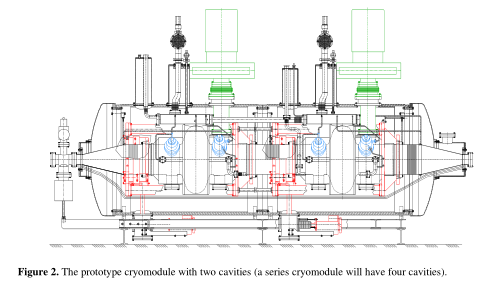
\includegraphics[width=1\textwidth]{figures/experiment/rfproto.png}
\caption{Schematic of a prototype RF cryostat, containing only two cavities. Figure from the The LHC Superconducting RF System \cite{boussard}.}
\label{fig:cavities}
\end{figure}

There are eight single-cell cavities per beam.
Four cavities are grouped to share a single cryostat, which maintains their superconducting temperature.
The resulting total voltage gradient is 16~MV per beam.
A simplified schematic is shown in Figure \ref{fig:cavities}.
The driving frequency is supplied through the couplings on top of the cryostat.
The cryostats are too large to sit next to each other in the tunnel, so they are staggered.

\subsection{Magnet Design}
If the accelerator is the heart of the LHC, the magnets compose its body.
Magnets serve multiple purposes in handling the beam.
\begin{itemize}
    \item Dipole magnets bend the beam around the curved sections.  There are 1232 main dipoles.
    \item Quadrupole magnets focus and defocus the beam. Each quadrupole simultaneously focuses in one direction and defocuses in an orthogonal direction. There are 392 arc quadrupoles throughout the LHC.
    \item Sextupole for correcting chromaticity introduced by quadrupoles. There are 2464 in total.
    \item Other magnets such as octupole and decapole correctors fill in the remaining 7000 superconducting magnets.
\end{itemize}
Together these magnets steer the beam into the LHC and maintain the beam's orbit during collisions.
At the end of the beam's lifetime, kicker magnets steer the beam safely into the beamdump.

\begin{figure}[h!]
\captionsetup[subfigure]{position=b}
\centering
\subcaptionbox{One element group\label{fig:dipoleFlux2}}{
    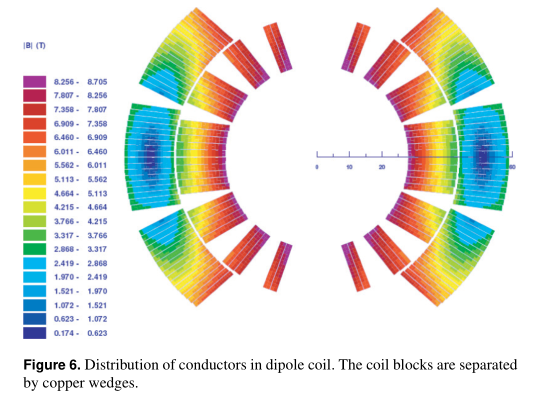
\includegraphics[width=0.4\textwidth]{figures/experiment/coils.png}
}
\subcaptionbox{One element group\label{fig:dipoleFlux1}}{
    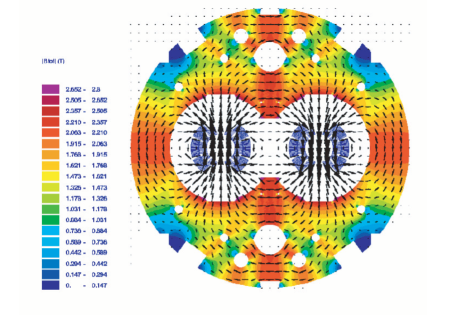
\includegraphics[width=0.4\textwidth]{figures/experiment/field.png}
}
\caption{Illustration of the magnetic flux in the dipole magnets. Figure from the The Large Hadron Collider \cite{lyndon}}
\label{fig:dipoleFlux}
\end{figure}

% Dipole system
The dipole magnets perform the job of bending the beam around the LHC.
Because the counter circulating beams are both positively charged, magnetic fields of opposite directions are needed to steer them.
In the dipole magnets, two sets of superconducting coils are wound from niobium-titanium (Nb-Ti) alloy wires\footnote{Although niobium-tin (Nb$_3$Si) has many desirable advantages over Nb-Ti, it is brittle and requires many hours of heat treatment at 970~k. On the other hand, Nb-Ti has a low heat capacity at 1.8~k, so it is susceptible to rapid heating and quenching}.
The coils are arranged in inner and outer layers, as shown in Figure \ref{fig:dipoleFlux2}.
This configuration produces a homogeneous, purely dipole field.
The coils for each beam are positioned side-by-side, such that the field of one can augment that of the other.
These coils share a common yoke made from low carbon steel with high magnetic permeability, chosen to conduct the magnetic flux between the coils.
This is illustrated by the black arrows in Figure \ref{fig:dipoleFlux1}.
The coil and yoke assembly is held in place by collar plates of austenitic (low permeability) steel.
The resulting magnetic field has an incredible strength of 8.3~T.
Each of the main dipole magnets has a length of 14.2~m (15~m, including connections between the magnets).

% Cryosystem
In order to operate at superconducting temperatures, the magnets are housed elaborate cryosystems.
These are challenging systems: during the LHC's Run 1, the cryosystem was responsible for 25-30\% of fault time.\cite{lhcRun1}
It is the task of the cryosystem to maintain the magnet at 1.9~k using superfluid helium. A total of 100 tons is used throughout the LHC.
Helium is used because its low viscosity allows it to permeate the coil insulation and contact directly with the superconducting wire.
Since the superfluid helium has a specific heat roughly 2000 times that of the Nb-Ti, this has the important benefit of increasing the system's specific heat.
Helium is also effective at quickly transporting heat away from the wired.
The magnets are submerged in a bath of 1~bar liquid helium. A pipe with is pumped with low pressure 15~mbar liquid helium to pull heat away from the bath.
This is done to prevent vapor bubbles from developing in the bath, leading to the coil heating and subsequent quenching.
In the event of a quench, a capacitor bank is fired into series with the coil to make it resistive. The current is diverted through a diode while the power is ramped down.

Magnets are grouped into ``periods'' with identical magnetic properties.
Each period is 106.9~m long and consists of six main dipoles and two 6.6~m ``short straight sections'' (SSS).
Each SSS contains quadrupole magnets that re-focus the beam after being steered by the dipoles.
Additionally, each SSS also contains sextupoles that control chromaticity and small dipoles for orbit corrections.
Some SSS also contain octupoles and trip/skew quadrupoles for fine-tuning the beam characteristics.
Perturbations in the trajectory of the beam are introduced by the magnets and are called \emph{dispersion}.
After completing one of the eight arcs, the magnet of the dispersion suppressor system cancels horizontal dispersion introduced by during the bending.

\subsection{Beam Structure and Design}
The achievement of building the LHC pales in comparison to the achievement of producing and maintaining its beams.
The LHC was designed to collide two counter-rotating beams, at precise locations, with the enormous instantaneous luminosity of $10^{34}cm^{-2}s^{-1}$.
The energy of each beam exceeds that of a large truck traveling at highway speeds.
This is more than one hundredfold the stored beam energy of any previous machine. \cite{lyndon}
The beam is an object of enormous energy and surpassing delicacy.
Numerous technical considerations must be addressed in order for the beam to be useful for the experiments.
The beams at the LHC are characterized by several parameters that describe its stability and utility.
These parameters are described in this section.

The first parameter to consider is the \emph{emittance}, $\epsilon$, defined in Equation \ref{eqn:emittance}.
It is a measure of the distribution of the particles in a beam in position-momentum phase space.
The emittance is defined as
\begin{equation}\begin{split}\label{eqn:emittance}
\epsilon \equiv \frac{6\pi}{B}\left(w^2-D^2\left(\frac{dp}{p}\right)^2\right),
\end{split}\end{equation} 
where $w$ is the RMS beam width, $D$ is the dispersion, $B\approx(w/\epsilon)$ is the beta function, and $\frac{dp}{p}$ is the relative momentum spread.
The emittance is often divided into longitudinal and transverse components.
If the emittance is too small, then intra-beam interactions destabilize the beam. 
During injection, the beam has a longitudinal emittance of 0.6-1 eV, and this is increased to 2.5 eV during acceleration for stability.
Conversely, if the transverse emittance is too large, colliding beams pass through each other without interacting.
\cite{boussard}\cite{lyndon}\cite{pdgAccelSection}

\begin{figure}[h!]
\captionsetup[subfigure]{position=b}
\centering
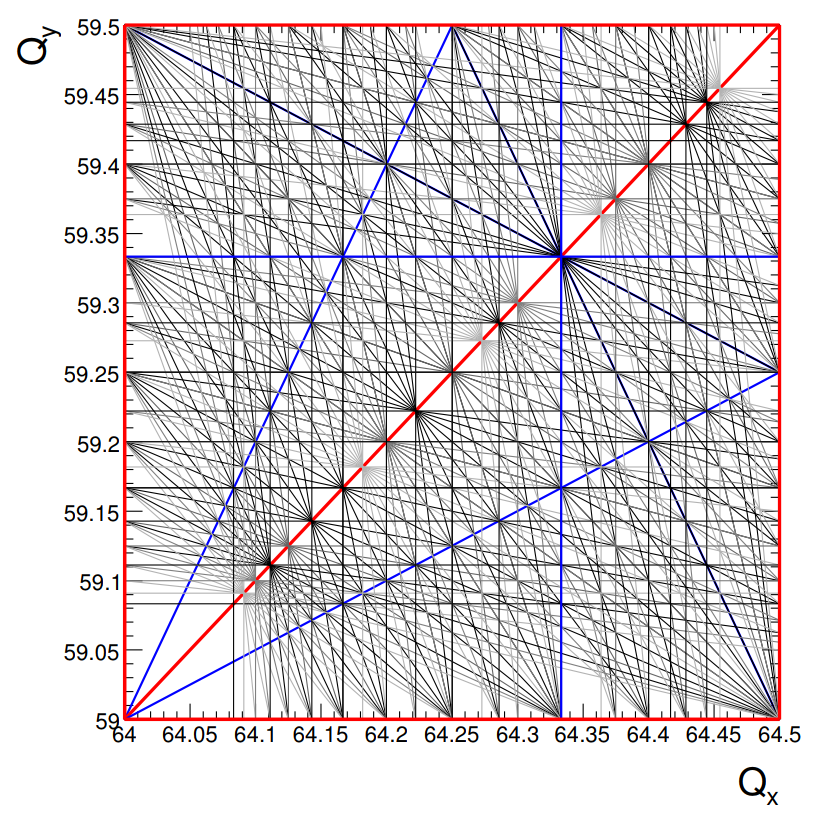
\includegraphics[width=0.4\textwidth]{figures/experiment/tune.png}
\caption{Tune diagram for the LHC. The horizontal and vertical tunes are displayed. First order resonances shown in red, second order resonances shown in blue, and higher order resonances shown in black. Figure from \emph{Tune and Chromaticity Diagnostics} \cite{steinhagen}}
\label{fig:tune}
\end{figure}

Related to the transverse emittance are \emph{betatron oscillations}: harmonic motion in the transverse plane as the beam makes an orbit.\cite{pdgAccelSection}
This is a problematic source of intra-beam scattering of protons through coulomb forces.
The frequency of betatron oscillations is higher than that of the orbit.
The number of vertical or horizontal betatron oscillations made during one orbit is called the vertical or horizontal \emph{tune}, respectively.
The horizontal and vertical tunes must be carefully picked using a tune diagram, as exemplified in Figure \ref{fig:tune}.
Resonances are illustrated as lines, and the tunes must be selected together to avoid disruptive resonances.
The beam density, $N$, as well as emittance and $\beta$ modify the tune tune $Q$:
\begin{equation}\begin{split}
    \delta Q\propto-\frac{N}{\beta\gamma^2\epsilon^*}.
\end{split}\end{equation} 
For example, when the PSB was renovated the emittance was reduced, and the energy ($\gamma$) was increased to compensate for the in on tune.
In practice, tunes are adjusted continually by adjusting these parameters throughout beam injection, ramping up beam energy, and eventual collisions.

Related to the longitudinal emittance are \emph{synchrotron oscillations}: longitudinal oscillations along the direction of the beam.
This takes place at a much lower frequency than that of betatron oscillations: at the LHC it is less than one oscillation per orbit.
As with betatron oscillations, the synchrotron oscillation frequency must be carefully controlled to limit intra-beam scattering and maintain beam stability.\cite{pdgAccelSection}

\emph{ chromaticity} describes the dependence of the tune on a change of momentum.
In optics, light rays of different wavelengths are focused differently by a glass focusing lens.
There is a persistent analogy between optics and beam dynamics (often called beam optics). Like light, beams are bent and focused by magnets. 
Particles with large momentum experience weaker focusing strength from focusing quadrupoles, a process called \emph{chromatic aberration}.
Chromaticity quantifies this momentum dependence.
To put it explicitly, chromaticity $Q'$ is the tune change $\Delta Q$ caused by a relative momentum change $\Delta p/p$. \cite{fuchsberger}
\begin{equation}
    \Delta Q = Q'\frac{\Delta p}{p},
\end{equation}
where
\begin{equation}
\begin{split}
    \frac{\Delta p}{p} = \frac{\Delta f/f}{\eta}; \quad\text{and}\quad \eta = \frac{1}{\gamma_r}-\alpha_c. \\
\end{split}
\end{equation}
Here, $\Delta f$ is change in RF frequency, and $f$ is the nominal frequency \footnote{400,788,860 Hz at the LHC.} 
$\gamma_r$ is relativistic gamma function, and $\alpha_c$ is momentum compaction factor equal to $3.225\times10^{-4}$ at the LHC.
Chromaticity is unitless as it defines a change in the tune.
At the LHC, sextupoles control the beam's correct chromatic aberration after passing through focusing quadrupoles and dispersion suppression. \cite{frascati} \cite{bruno}
The chromaticity is visualized on a tune diagram, such as Figure \ref{fig:tune}, as the area occupied by the beam.
Reducing the beam's chromaticity makes it easier to find a stable setting for the tune.
% From Jorg
However, beams with a chromaticity that is too small suffer from instability related interaction with the beampipe.
The momentum spread of a beam with high chromaticity makes it more efficient to absorb reflected EM fields without perturbing the beam.
An important task is to find a balance for the chromaticity in order to maximize the useful life of the beam.

% Bunches
Because the RF cavities produce alternating field gradients, the beam is naturally organized into occupied \emph{bunches} and empty space.
The time interval between these, the bunch spacing, is a multiple of the RF frequency.
At the LHC the nominal bunch spacing is 24.96~ns, or ten times the RF frequency. The corresponding bunch length is 7.5~cm. \cite{boussard}
Bunches are collected into trains, patterns of occupied and empty bunches.
Several trains comprise the beam.
Several bunches are always left unoccupied, called the abort gap. The length of the gap corresponds to the ramp time of the extraction kicker magnet.
The bunch design choice depends on the function of the beam. Some patterns are useful for cleaning the beampipe of electron clouds, while others are useful for optimizing physics collisions.

% Lumi
From a physics perspective, the most important beam characteristic is the instantaneous luminosity of collisions.
This is defined as $L\equiv N/\sigma_{pp}$, where $N$ is the collisions per second and $\sigma_{pp}$ is the poorly defined proton-proton collision cross-section\footnote{This is poorly defined because in some sense protons always scatter off each other, so the definition depends on what constitutes a collision. Traditionally, values of $\sigma_{pp}\sim10^{14}\text{fb}$ are used.} \cite{lyndon}
More precisely in the context of the LHC, the luminosity is defined in Equation \ref{eqn:lumi}.\cite{lyndon}
\begin{equation}\label{eqn:lumi}
    L=\frac{N_b^2nf_r\gamma}{4\pi\epsilon_n\beta^*}
\end{equation}
Here, $N_b$ is number of particles per bunch, and $n$ is the number of bunches per beam.
$f_r$ is is revolution frequency, which is 11.245 kHz for the LHC.
The other terms are the previously mentioned relativistic $\gamma$, the transverse emittance $\epsilon_n$, and the beta function at the collision point $\beta^*$.
The two beams must be steered into each other at a crossing angle of $\theta_c$.
This results in a luminosity reduction factor,
\begin{equation}\label{eqn:lumiReduce}
    F=1/\sqrt{1+\frac{\theta_c\sigma_Z}{2\sigma^*}}
\end{equation}
where $\sigma_z$ is the RMS bunch length, and $\sigma^*$ is the transverse RMS beam size at the interaction point.
In fact, $\sigma^*$ is specifically minimized by focusing the beam before the collisions and defocusing it afterward.

The challenge during the operation of the LHC is to keep the beam in a stable orbit for many hours.
A number of issues can affect the stability of the beam during this time. \cite{lyndon}
\begin{itemize}
    \item \textbf{Beam-beam interaction:} the force from the electromagnetic field from one beam on another. Beam-beam interaction can be reduced by increasing the crossing angle of $\theta_c$, but this reduces the luminosity, as shown in Equation \ref{eqn:lumiReduce}.
    \item \textbf{Intra-beam interaction:} coulomb scattering during betatron and synchrotron oscillations. While protons migrate within a bunch, they can knock other protons into different betatron orbits. At the LHC, intra-beam leads to a growth in horizontal emittance of 0.3-0.5~$\mu$m/hour.
    \item \textbf{Coherent instabilities:} the beam interacts with its environment, generating EM fields, that in turn, act on the beam. The induced fields are mitigated by smoothing the beampipe as much as possible, to the extent where interconnects are covered with smooth segments. The impact of coherent instabilities on the beam is decreased by increasing chromaticity.
    \item \textbf{Electron clouds:} (e-clouds) the accumulation of electrons in beam pipe. The major sources are ionizing the residual gas in the beam pipe and excitation from synchrotron radiation knocking electrons off the beam pipe. The issue is that the beam can collide with these free electrons and accelerate them. The energetic electrons collide with the beampipe and produce an electron shower, leading to an exponential growth of the cloud. This is especially problematic if the mean drift time for electrons is resonant with beam bunch spacing. E-clouds are a large source of heat for the cryogenic equipment. E-clouds are combatted by improving the vacuum and picking bunch structures that do not resonate with the clouds. As a further measure, warm chambers (including in the detectors) are coated with TiZrV, a ``getter'' material that passively pumps vacuum and absorbs electron clouds.
\end{itemize}


\subsection{Beam Abort}

\begin{figure}[h!]
\captionsetup[subfigure]{position=b}
\centering
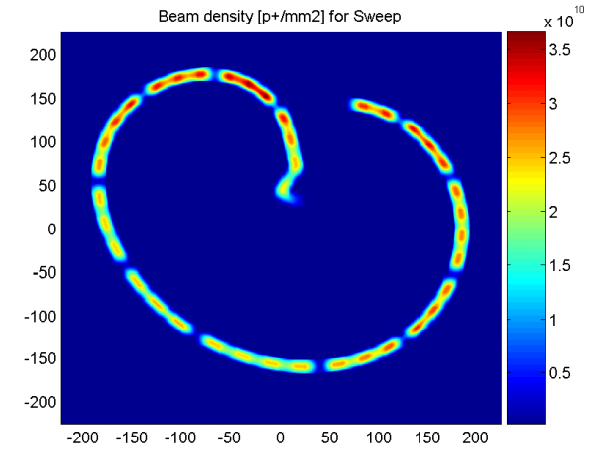
\includegraphics[width=0.5\textwidth]{figures/experiment/beamdump.png}
\caption{The trace of the beam across the beam dump TDE. Figure from A Large Diameter Entrance Window for the LHC Beam Dump Line \cite{beamdump}.}
\label{fig:beamdump}
\end{figure}

When the beam has degraded to the point where it is no longer useful, it must be disposed of safely.
Over the course of several hours, the beam loses intensity to the point where it is more efficient to dump the beam and replace it.
Occasionally an error in one of the LHC subsystems will be detected, and the beam is dumped as a precaution.
In both cases, the beam dump system is used to remove the beam from the machine while minimizing damage to its components.

There are three steps in disposing of the beam. 
The first is to extract the beam from its nominal orbit.
The second is to dilute the beam's density.
Finally, the beam is absorbed in a material, where its energy is converted to radiation and heat. \cite{lhcDesignV1}

Focusing on one beam, it begins in its nominal orbit, when an abort is triggered. 
If the beam is in a safe state, the abort system will wait until the abort gap arrives to ramp up the extraction kicker magnets (MKD).
If the beam needs to be dumped immediately, the MKDs can ramp up outside the abort gap with minimal damage to the system.
The 15 copper wound magnets are powered by a bank of capacitors that can quickly energize the magnets in under 3.0~$\mu s$ to produce a field of 0.34~T. 
Once energized, the MKDs deflect the beam horizontally out of the ring.
The magnets remain on for 90~$\mu s$ to allow the full beam to exit the ring.

Next, the diluter kicker magnets (MKB) sweep out the beam in an ``e'' pattern, as shown in Figure \ref{fig:beamdump}.
This spreads out the area where the beam will deposit its energy.
The diluter is built from four horizontal and six vertical magnets powered by a sinusoidal current to produce the shape.
Like the MKDs, the MKBs are non-superconducting low-oxygen copper wound magnets.

The Extraction Septum Magnets (MSD) have a septum (gap) for the extracted beam.
A low-field hole is drilled through the yoke to allow the passage of the circulating beam.
The MSDs are responsible for deflecting the beam vertically.

Finally, the beam comes to the Beam Dump Absorber Block (TDE).
This consists of carbon cylinders due to its high melting temperature and thermal shock resistance.
In particular, alternating layers of solid polycrystalline graphite cylinders and flexible graphite are used to balance solidity and flexibility.
The total length of the carbon material is 7.7~m long.
The TDE is kept at atmospheric pressure. This raises the question: how is the TDE isolated from the vacuum of the beamline? A low-Z carbon composite layer is used to separate the two, while a thin layer of vacuum insulation prevents small leaks. \cite{beamdump}
The TDE jacket is cooled by water pipes to help reduce the thermal stress on the carbon.
Finally, the assembly is surrounded shielding made from old dipole yokes filled with concrete.

The MKD and MSD magnets used in the beam abort share a design with the magnets used to steer the beam into the rings during injection.
At the beam dump, the MKDs deflect horizontally while the MSDs deflect vertically.
At the injection points, it is reversed, and the MKDs steer the beam horizontally while the MSDs steer it vertically.


\subsection{History of the LHC}
The history of physics runs of LHC is the description of the laboratory conditions under which ATLAS collected data.
It is also an interesting narrative of a tightly coupled process of developing and testing collider engineering principles.
The dramatic improvement of the machine's performance over the years of its operation is a testament to the efficacy of this strategy.

This section will first describe the LHC's first round of operation, Run 1.
During Run 1, the physics discovery was made that motivates the search for \vhmm reported in Chapter \ref{sec:hmumu}.
Crucial machine developments were also made in Run 1 that lead to energy and luminosity increases during Run 2, enhancing the precision of the non-resonant search reported in Chapter \ref{sec:ci}.
This section proceeds to describe the second round of operation, Run 2.
During Run 2, the machine provided collisions based on the data used for this thesis.

\subsubsection{Run 1}

The first run of the LHC took place between 2010 and 2013.
Collisions took place with beam energies between 3.5 and 4~TeV.\cite{lhcRun1}
Run 1 provided the collision data in which the Higgs boson was discovered. \cite{atlashiggs}
It also provided the basis for the steady improvement of the LHC.
For example, as a result of the experience gained from operating the machine, it was possible to gradually decrease the bunch spacing from 150~ns (2010), to 75~ns (2011) finally to 50~ns (2011/2012). \cite{lhcRun1}

The run began in 2010 with counter-rotating beams of energy 1.2~TeV.
This energy, which is below the design energy of 7~TeV per beam, was selected due to earlier damage during operation in 2008.
After verifying the stability of the machine, the energy was gradually increased to 3.5~TeV per beam.
The first physics ready collisions began on February 27, with just two bunches per beam and containing relatively few protons each.
Over several months, the number of bunches and the number of particles per bunch were increased.
The operation was not without difficulty: throughout the run, unidentified falling objects (UFOs) within the beam-pipe disrupted the beam and resulted in 60 beam dumps.
The UFO events are speculated to be caused by water vapor solidifying on the top of the beam-pipe and later fall through the beam.
Furthermore, unexplained and mysterious oscillations in the beam tune (called the ``hump'') plagued operators. \cite{lhcRun1}
The year ended with significant gains in the beam energy, bunch spacing, and bunch density.

The second year of the run began on February 19, 2011, with three weeks of recommissioning.
The first physics beams began on March 13 at 3.5 TeV and 32 bunches per beam.
This was gradually increased to 200 bunches, with 75~ns spacing.
The bunch density was also increased to 1.34$\times10^{11}$ ppb.
On April 21, the LHC reached an instantaneous luminosity of $4.6\times10^{33}~\cms$, which broke the previous record from the Tevatron.
It is at some time during 2011 that the hump disappeared from the tune plots, leaving the mystery unresolved.
Overall, the second year was the first to provide productive physics data. The mean stable beam time was 6.1 hours, which corresponds to 33\% efficiency.
In total, 5.6~\fb of data was provided. \cite{lhcRun1}

In the years 2012 and 2013, the investment in carefully developing the LHC paid off with a wealth of physics data.
The beam energy was increased to 4~TeV in order to increase the Higgs production cross-section.
The first stable beams at 4~TeV, holding only three bunches, were circulated on April 5, 2012.
After a month of commissioning, the first physics beams were provided on May 4.
The nominal beam design was 1374 bunches with 50~ns bunch spacing\footnote{Due to the arrangement of the bunches, only 1368 bunches collided inside ATLAS. At the time, there was also a plan to have private bunches colliding only in LHCb.}.
The bunch intensity was also increased to 1.7$\times10^{11}$ ppb, and the run stable beam efficiency was improved to 36.5\%.
% Emittance 2-2.5 microns

\begin{figure}[h!]
\captionsetup[subfigure]{position=b}
\centering
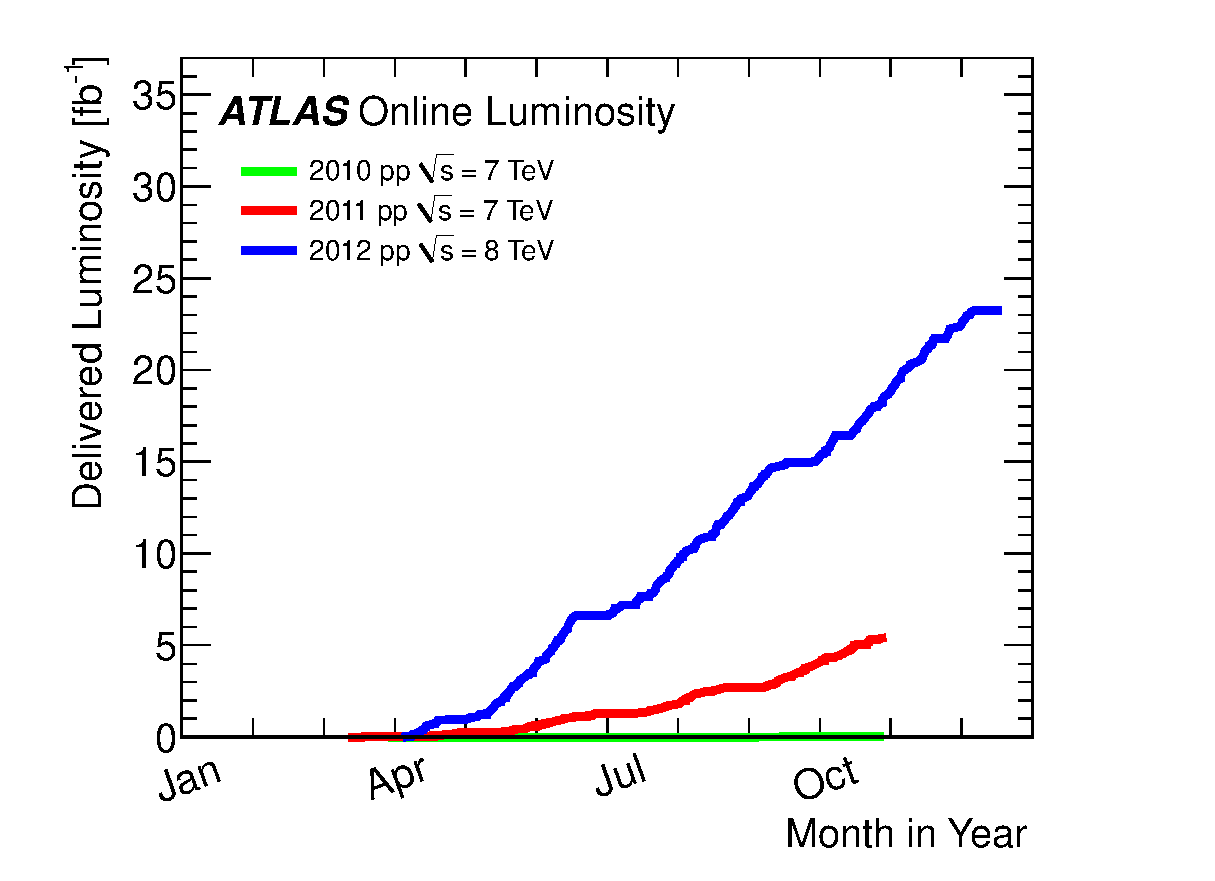
\includegraphics[width=0.8\textwidth]{figures/experiment/lhc/run1Lumi.eps}
\caption{ (from: https://twiki.cern.ch/twiki/bin/view/AtlasPublic/LuminosityPublicResults)}
\label{fig:run1Lumi}
\end{figure}

The performance of the LHC during Run 1 enjoyed dramatic improvement over time.
This is evident in Figure \ref{fig:run1Lumi}, which shows the integrated luminosity for various years, as recorded by ATLAS.
The rate at which the machine delivered data grew steadily due to the iterative study and tuning that took place during Run 1.
However, the machine operation was far from perfect, and the cryogenic system was most problematic, causing 25-30\% of all downtime, followed by the injector systems.
Resolving these issues was a major goal for Run 2. \cite{lhcRun1}

    % \item \textbf{Beam Cycle} (probably, should use run2 resource) \cite{lhcRun1}
    % \begin{itemize}
    %     \item Injection. Beam is ``scraped'' by transfer line collimator's. In run 1, about 2-4\% of the beam is lost. This done in SPS. The collimator jaws heat and outgas, so these are opened as soon as injection is finished. Rings are filled consecutively (as opposed to alternating bunches) because ALICE requested it (it reduces their background??). \cite{lhcRun1}
    %     \item Ramp. The ramping speed is limited by dipole current ramp rate of 10 A/s, which corresponds to 6 GeV/s. A ``flat top'' of 300 s, during which the tune decay is corrected for. \cite{lhcRun1}
    %     \item Separation/crossing angles. {\color{red} Warning, confused} Crossing angle is 170 micro radians. Separation is on the order of mm. Horizontal separation in P1,P2. Vertical in P5,P8. Hence in IR1 beam 1 moves downward/inside. \cite{lhcRun1}
    %     \item Collisions. When start, tails of bunches are expelled, leading to a brief drop in expected beam lifetime. The expected lifetime of the beam is optimized by reducing the chromaticity {\color{blue} \url{https://cds.cern.ch/record/302491/files/p77.pdf}(the change in linear parameters of transverse motion with beam energy).} HOW do they reduce chromaticity? \cite{lhcRun1}
    %     \item Tune. The beam is large during the ramp, and reduced during squeeze. \cite{lhcRun1}
    %     \item Collimators. Used for squeeze, used for betatron cleaning. Used to clean ``physics debris''. \cite{lhcRun1}
    % \end{itemize}
% \end{itemize}

\subsubsection{Run 2}

The second operation of the LHC took place between 2015 and 2018.
This run is characterized by higher beam energy: 6.5~TeV per beam throughout the run.
This is a monstrous amount of energy to concentrate into the protons that make up the beam.
To perform this feat with AA batteries, a proton would have to be transported down a stack that reached from Earth to the sun and then on to Mercury.
It is also characterized by innovative strategies to increase the delivered luminosity.
Key among these improvements are a small emittance and $\beta^*$ and reduced 20~ns bunch spacing.

The machine cycle begins with threading: the beam is injected with low bunch intensity and stopped on collimators at stages throughout the rings.
The trajectory is adjusted at each stop before proceeding to the next one.
Threading takes place primarily at the beginning of the year since fewer corrections are needed when the machine is in a steady state.
When a complete orbit can be made by a 12-bunch beam, the position of several orbits is averaged, and then adjusted, in a process called steering.
When the orbits are stable, the rest of the beam is injected \footnote{This is done sequentially, rather than simultaneously, for each beam. This is because simultaneous injection heated the injection collimators, causing them to off-gas.}.
When the complete beam has been injected, it undergoes a combined \emph{ramp and squeeze}\footnote{Combining ramp and squeeze was an innovation to increase the beam-on efficiency. Previously the squeeze was performed after ramping.}.
During ramp, the beam is accelerated while the dipole magnets simultaneously ramp up their fields.
The standard ramp time is 1210s. 
The ramping pattern is parabolic-exponential-linear-parabolic and takes approximately 20 minutes. 
During the squeeze, the beam optics are adjusted in steps to reach a particular $\beta^*\approx30$~cm target in the interaction regions.
The squeeze continues after the ramp.
Once it is complete, the beams are steered to collide.

During the whole process, the beam tune and chromaticity are delicately adjusted.
For example, the chromaticity is controlled to $\pm$2 during filling and has typical values of +20 during filling and +15 during operation. \cite{lhcRun2}
The positive chromaticity enhances beam stability, in particular head-tail instability within bunches.
% The SPS bunch spacing is 200-250~ns.

It is desirable to maintain a target luminosity (1.5\times{34}\cms), with a process called luminosity leveling.
This is accomplished by adjusting the crossing angle $\theta_c$ (introduced in 2017), and the value of $\beta^*$ (introduced in 2018).
Since the beam is extremely sensitive to perturbation, these adjustments are made in small steps of 10 micro radians, and $\approx3$~cm.
The beam is so sensitive to external sources that tidal effects, earthquakes, and HL-LHC civil engineering have all been observed in the radial orbit evolution over time, as shown in Figure \ref{fig:tides}.

\begin{figure}[h!]
\captionsetup[subfigure]{position=b}
\centering
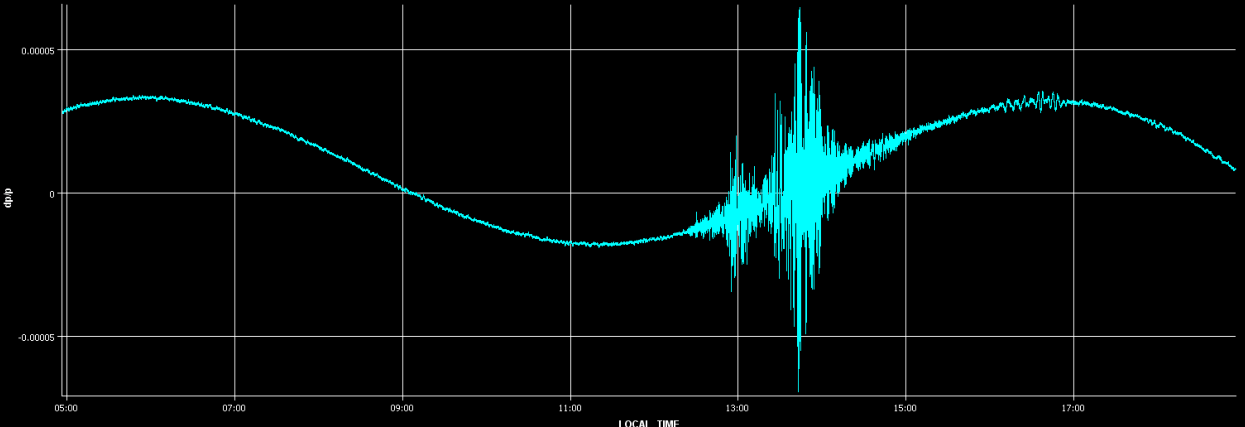
\includegraphics[width=0.99\textwidth]{figures/experiment/lhc/tides.png}
\caption{The evolution of the radial orbit $dp/p$. The LHC ring distorts under tidal forces, which is seen in the long period oscillation. The effect of an earthquake in New Zealand appears just after 13:00. Figure from Operation and Configuration of the LHC in Run 2 \cite{lhcRun2}}
\label{fig:tides}
\end{figure}

The first 6.5~TeV beams with 25~ns bunch spacing arrived on April 5, 2015.
After a brief commissioning period, the first stable beams were delivered on June 3.
The run began with a conservative $\beta^*=80$~cm.
Luminosity increased throughout the year, with beams of 2244 bunches per beam contributing to a peak instantaneous luminosity of $5.0\times10^{33}\cms$ by the end of the year.
In all, the LHC delivered 4.2~\fb of physics collisions to ATLAS during 88 days in 2015.
This was constrained by a large heat load due to unexpectedly intense electron clouds, which saturated the cryosystems' cooling ability.
The e-clouds are problematic and lead to an emittance growth of 0.6~$\mu$m/hour.
Low-intensity beams were used in an effort to push the e-clouds out of the beam pipe (scrubbing), but these were ineffective.
A particularly bad incident took place in Beam 2 (15R8), where a UFO blocked a large portion of the beam pipe.
It was suspected that this was a piece of ice, so the beamscreen was heated to 80~k, but again this was ineffective.
Eventually, the beam was steered around the object (called the ULO, or unidentified lying object).
The object remained in place for the full duration of Run 2, occasionally changing shape.
Eventually, when the machine was opened at the end of the run, the ULO was discovered to be a piece of plastic wrapping, possibly from installation.

Beams arrived the following year on March 25, 2016, with an ambitious target of $\beta^*=40$~cm and 25~ns bunch spacing.
During commissioning, the number of bunches per beam was steadily increased to 2220.
Physics beams arrived on June 26, and with that, the LHC finally delivered its design instantaneous luminosity of $1.0\times10^{34}\cms$.
Improvements over the year include a new bunch preparation and reduced transverse beam size, leading to a peak luminosity of $1.4\times10^{34}\cms$. \cite{lhcRun2}
Unfortunately, CMS received 5-10\% more collisions due to the collision geometry. \footnote{The crossing plane for ATLAS is vertical, while for CMS, it is horizontal. The early 2016 beams were oblong with low vertical emittance, leading to a more favorable luminosity reduction factor for CMS (Equation \ref{eqn:lumiReduce}).}
The year concluded with the only major problem being an August 10 short circuit in a sector 12 dipole magnet, which required replacement\footnote{This is aside from the problem where a beech marten chewed through a transformer cable at p8, leading to several days of shutdown.}.
A record 38.5~\fb of physics collision was delivered during 146 days to ATLAS in 2016.

One of the key improvements introduced during 2016 was the new bunch preparation, \emph{Batch Compression Merging and Splitting} (BCMS).
The beam from Linac 2 is continuous, but the subsequent machines, starting with the PSB, accelerate bunches of protons. \cite{freyermuth}
To increase the throughput of the PSB, each of its four rings can be \emph{overfilled} by injecting the Linac 2 beam in different positions.
Overfilling increases emittance, which limits the output luminosity that can be achieved with this strategy.
%Nominal scheme
The ``nominal'' scheme to fill the PS from the PSB was to inject six bunches.
Each bunch is longitudinally split into three bunches, then by two, and again by two, resulting in a total 72 bunches. \cite{freyermuth}
%BCMS scheme
The BCMS scheme changes two things.
First, the overfilling of the PSB is reduced to two cycles.
Next, 8 (instead of 6) bunches are injected into the PS.
This reduces the emittance in the PSB, since the required intensity is lower, and injection is spread out over fewer turns.
The eight bunches are merged to four, then split by three, then two, then two.
This totals in 48 bunches, which means more cycles are needed to fill LHC.
This is offset by the gain from reducing transverse emittance and therefore increased luminosity. \cite{freyermuth}

The next year began with additional commissioning due to the replaced dipole.
The first beams were injected on April 29, and physics beams were delivered on May 23 with 2556 bunches per beam.
During commissioning, a problem in 16L2 lead to losses and unusual background radiation caused by e-clouds.
This was caused by air that had leaked into the vacuum and condensed during the magnet replacement.
An attempt was made to evaporate the gas by heating the beam screen to 80~k, but this exacerbated the problem.
Eventually, a bunch pattern (8b4e: eight bunches, four empty) designed to scrub the e-cloud was adopted with acceptable results.
Beginning in August, a full luminosity version of 8b4e was adopted.\cite{lhcRun2}
Despite this setback, a more aggressive squeeze down to $\beta^*=30$~cm resulted in a luminosity record of $2.1\times10^{34}\cms$.
This is too high for ATLAS data collection, so it was leveled to $1.5\times10^{34}\cms$.
A new record of 50~\fb of collisions was delivered over 140 days in 2017.\cite{lhcRun2}

An essential improvement introduced in 2017 is luminosity anti-leveling by adjusting the crossing angle.
The beam crosses the interaction point at an angle of $\theta_c$.
This leads to a 30-40\% loss in luminosity. \cite{gorzawski}
Prior to 2017, the beam angle was set based on the initial intensity of the beams. \cite{gorzawski}
Reducing the crossing angle as the beam intensity decays can help recover some of the delivered luminosity.
A study was conducted during a machine development period, using standard physics setup and few bunches. \cite{gorzawski}
The leveling is performed slowly over the course of several minutes in steps of 20-85 microradians.
This resulted in a gain of 3-4\% integrated luminosity per fill.

The first beams of 2018 were injected on April 30, and physics beams arrived ahead of schedule on May 17.
Despite efforts to heat the beam pipe during the shutdown, the 16L2 problem persisted\footnote{In fact, heating the pipe seems to have enhanced the problem. An estimated 0.1 gram of water vapor remained in each beam line.}.
As the year progressed, low intensity 900 bunch beams were used after a fill to reduce the e-clouds.
It is also remarkable to note that $\beta^*$ reached $25$~cm during collisions.
This final year of Run 2 benefited from previous years' development and successfully delivered 66~\fb of collisions during 145 days.


\begin{table}[htp]
\begin{center}
\caption{Summary of the beam conditions during Run 2. \cite{lhcRun2}}
{
\begin{tabular}{l r r r r r}\toprule
Parameter & 2015 & 2016 & 2017 & 2018  \\
Maximum bunches per beam                 &2244 &2220 &2556 &2556 \\
Emittance ($\mu$m)                       & 3.5 & 2.2 & 2.2 & 1.9 \\
$\beta^*$ (cm)                           & 80  & 40  & 30-40 & 25-30 \\
Total beam energy (MJ)                   & 280 & 270 & 330 & 320  \\
Average stable beam (hours)              & 6.8 & 11.2& 8.2 & 8.3  \\
Delivered integrated luminosity (\fb)    & 4.2 & 38.5 & 50  & 66   \\
Instantaneous luminosity ($10^{34}\cms$) & 0.5 & 1.4 & 2.1 & 2.1  \\
Average pile-up                          & 13  & 25  & 38  & 37   \\
Stable beam efficiency (\%)              & 35  & 49  & 49  & 49   \\
\bottomrule\end{tabular} %remember cline{1-2}
}
\label{tab:run2}
\end{center}
\end{table}

\begin{figure}[h!]
\captionsetup[subfigure]{position=b}
\centering
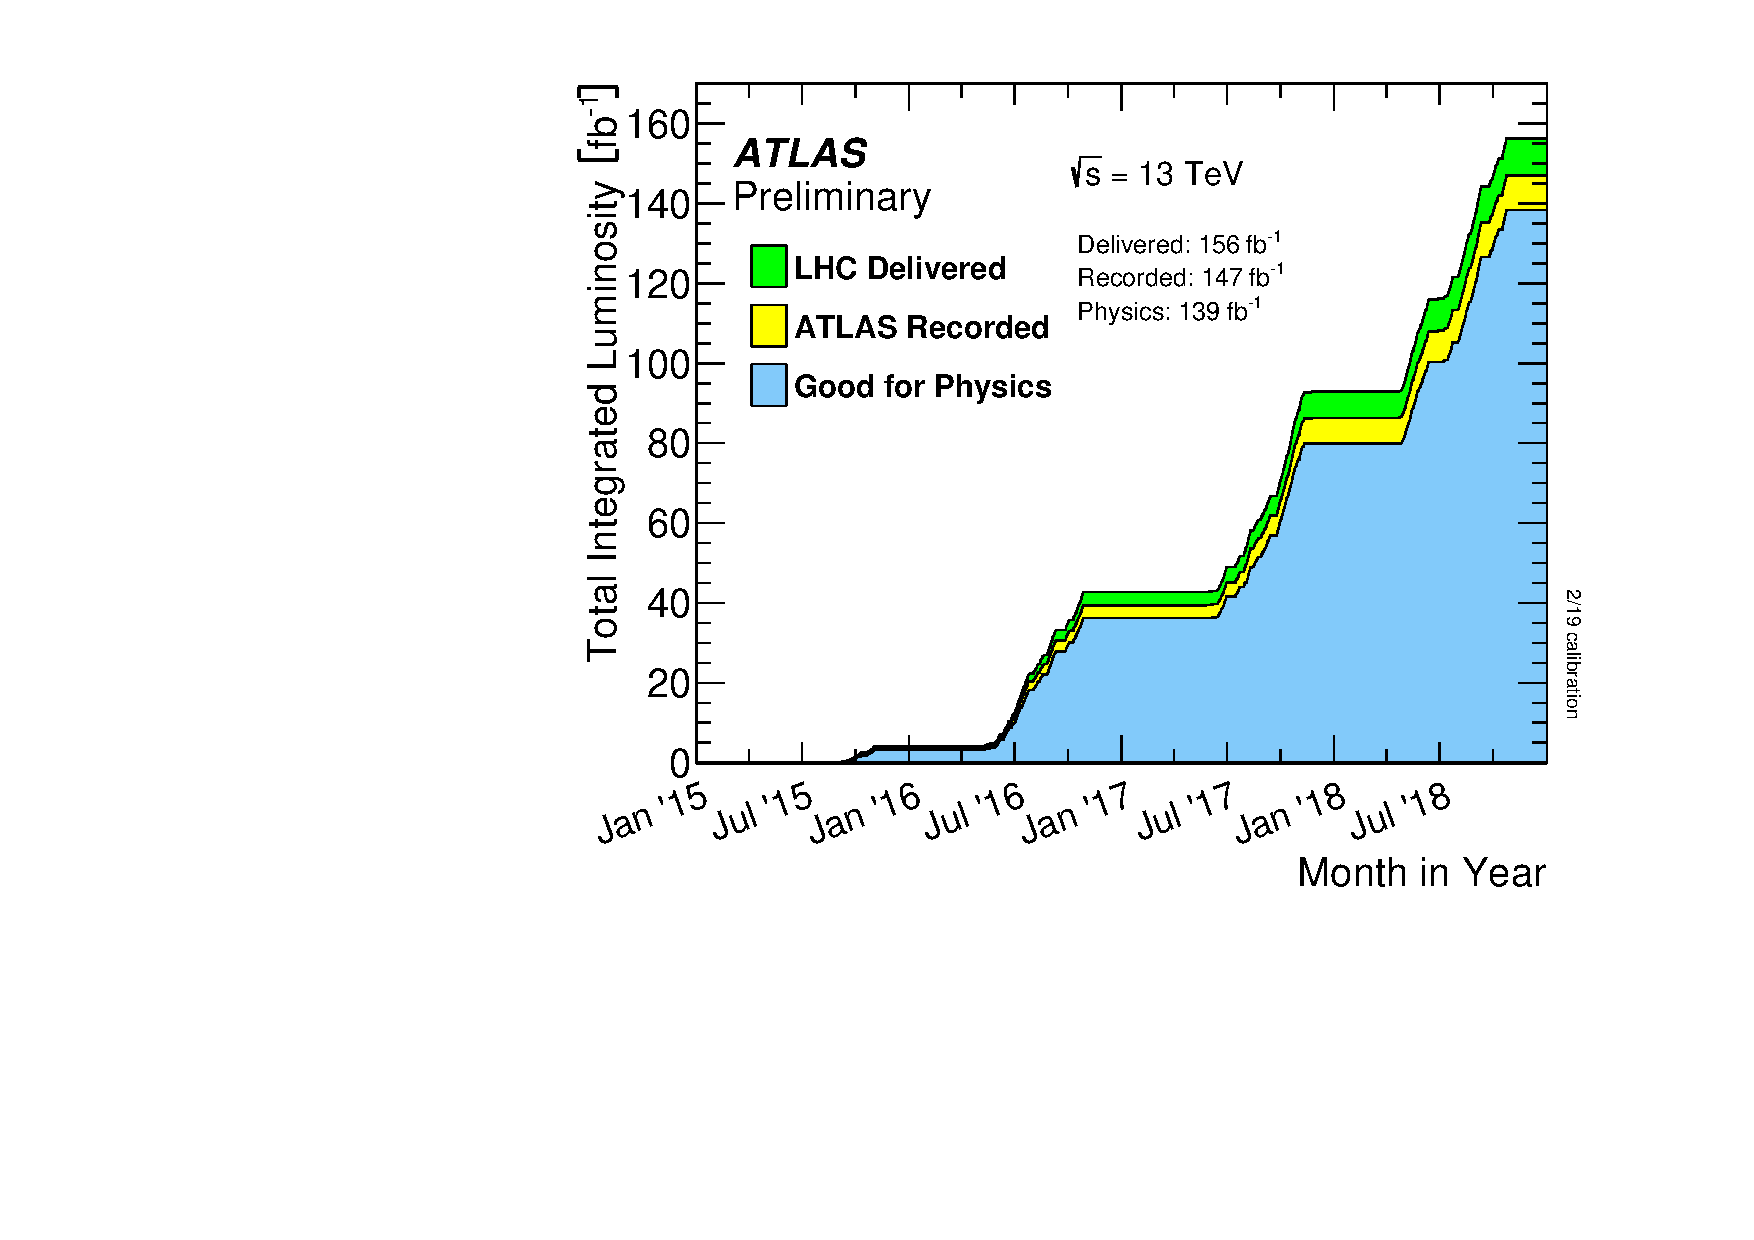
\includegraphics[width=0.8\textwidth]{figures/experiment/lhc/run2Lumi.pdf}
\caption{ (from: https://twiki.cern.ch/twiki/bin/view/AtlasPublic/LuminosityPublicResults)}
\label{fig:run2Lumi}
\end{figure}

The performance of the LHC during Run 2 enabled the machine to deliver a total of 156~\fb of collision data.
The total delivered integrated luminosity and that recorded by ATLAS are shown in Figure \ref{fig:run2Lumi}.
The number of commissioning days at the start of each year dropped from 58 down to 17, as the LHC was better understood.
Local optical corrections could be reused from year to year.
The maximum of bunches increased from 2244 up to 2556 per beam, and the stable beam efficiency increased from 35\% to 49\%.
During the run, UFO events occurred at rates of 1-20 per hour.
These and other run parameters are summarized in Table \ref{tab:run2}.
